\chapter{Efeito da ureia}
	\section{Motivação}
	A ureia demonstrou um comportamento que divergiu bastante dos outros aditivos. Por esse motivo, ela será estudada um pouco mais profundamente. Porém, a ação do salicilato de sódio não receberá muito enfoque, para simplificar o sistema. Portanto, foi estudado principalmente o efeito da ureia em soluções de CTAB, TTAB e DTAB, com concentrações diferentes de ureia e de surfactante.
	
	Ocorre a formação de um precipitado esbranquiçado em soluções de surfactante em concentrações maiores que 35\% de ureia. Isso ocorre a temperatura ambiente. Quando a solução é aquecida acima de cerca de 35ºC, ela se torna transparente. Esse comportamento foi estudado, variando-se o surfactante, sua concentração, e a concentração de ureia. Desses sistemas, foram estudadas as características térmicas, a estrutura da mesofase, e a reologia da fase esbranquiçada.
	
	\section{Calorimetria diferencial de varredura (DSC)}
		% todo: colocar o número da figura
		Foram preparadas soluções de ureia, em várias concentrações, com três surfactantes (CTAB, TTAB e DTAB), em três concentrações. Os termogramas resultantes foram organizados em figuras de modo a facilitar comparações. A tabela \ref{tab:refs_DSC} lista as comparações realizadas e em quais figuras estão.
		
		\begin{longtable}[h]{c c c}
			\toprule
			Conc. Surfactante \mM     & \% Ureia		& Figura 			\\
			\midrule
			CTAB 100	  & 38--45			& \ref{fig:DSC_CTAB_UR38-45}	\\
			CTAB 100, 200, 300	& 45, 40	& \ref{fig:DSC_CTAB_UR40-45}	\\
			TTAB 100, 200, 300	& 45, 40	& \ref{fig:DSC_TTAB_UR_40-45}	\\
			DTAB 100, 200, 300	& 45, 40	& \ref{fig:DSC_DTAB_UR_40-45}	\\
			CTAB, TTAB, DTAB 100	& 45	& \ref{fig:DSC_Surf_100mm_45p}	\\
			CTAB, TTAB, DTAB 200	& 45	& \ref{fig:DSC_Surf_200mm_45p}	\\
			CTAB, TTAB, DTAB 300	& 45	& \ref{fig:DSC_Surf_300mm_45p}	\\
			\bottomrule
			\label{tab:refs_DSC}
			\caption{Amostras analisadas e suas respectivas figuras}
		\end{longtable}
		
		\begin{figure}[h]
			\centering
			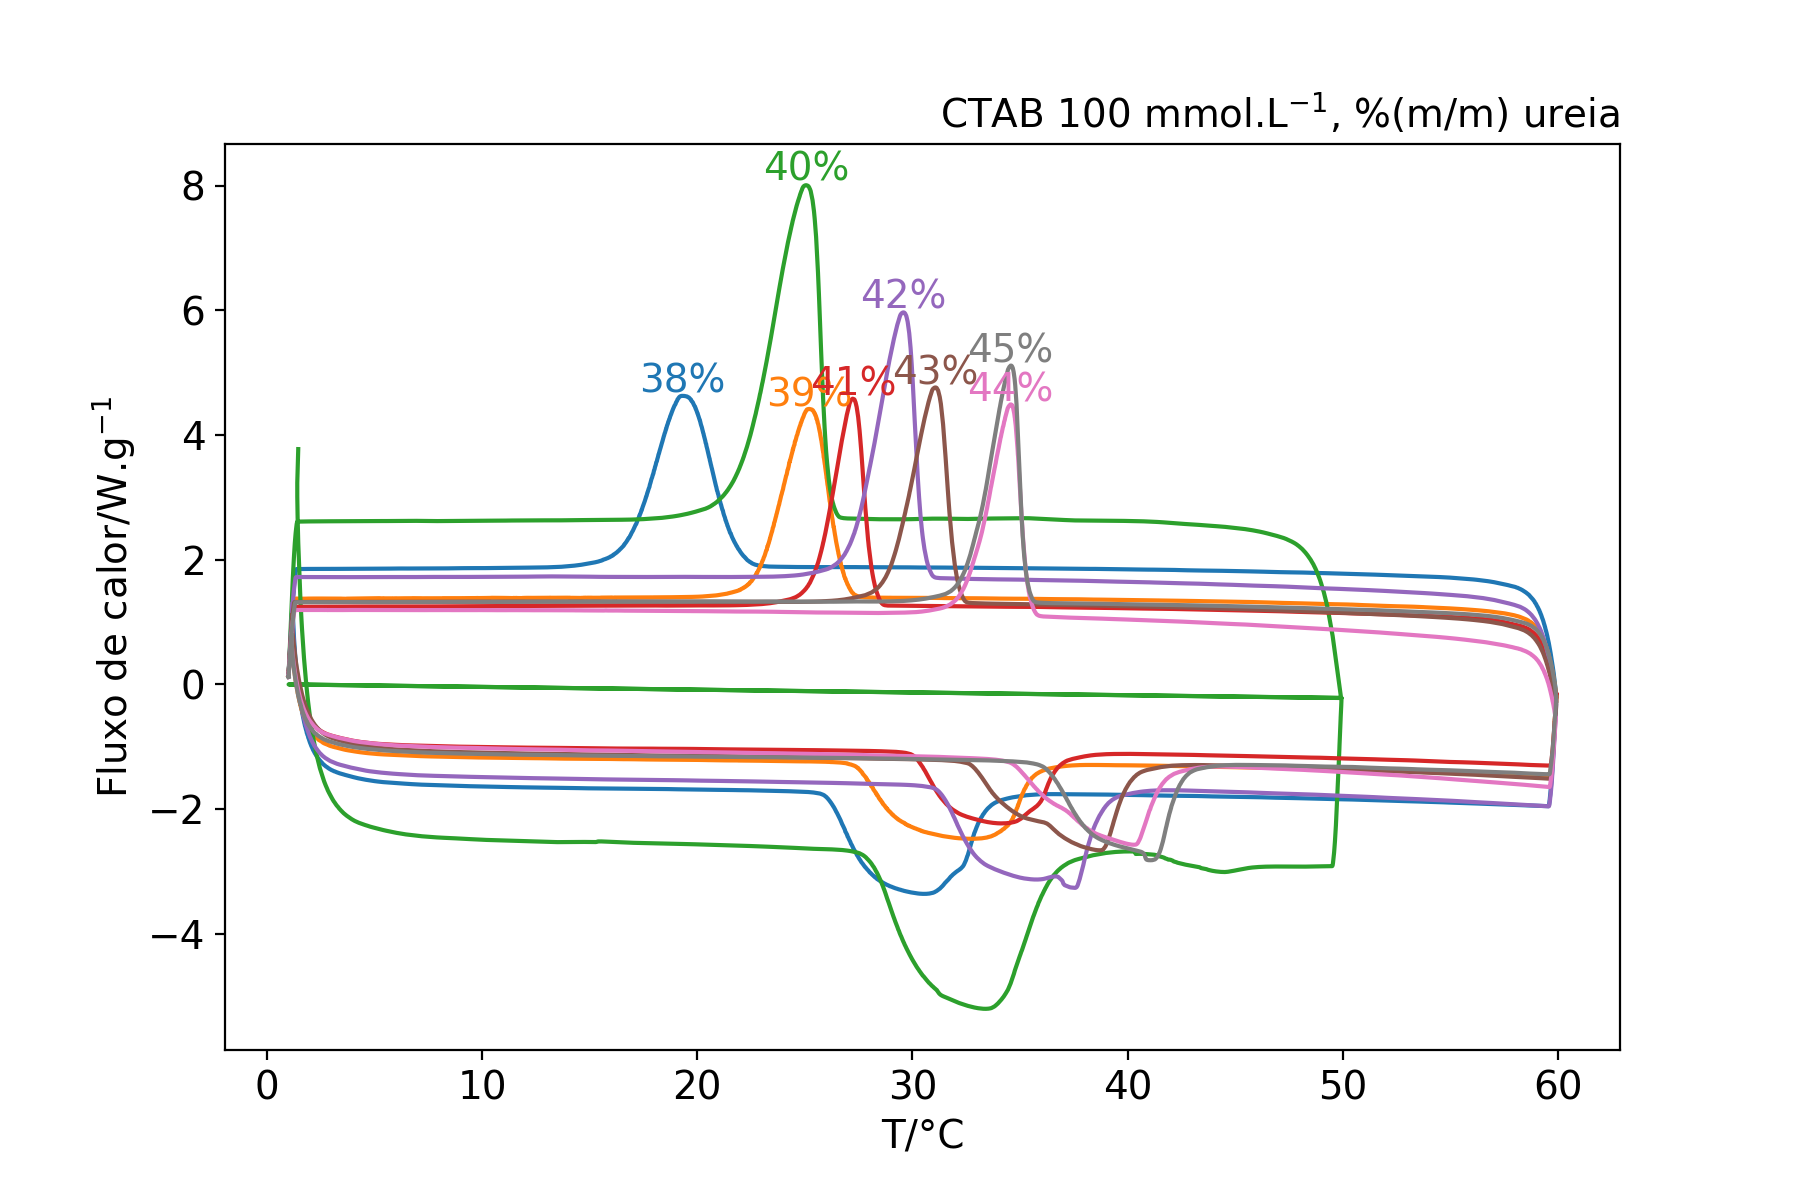
\includegraphics[width=0.75\textwidth]{./imagens/dsc/CTAB_porc_ur}
			\caption{Termogramas de soluções de CTAB 100 \mM{} em concentrações crescentes de ureia, de 38\% m/m a 45\% m/m}
			\label{fig:DSC_CTAB_UR38-45}
		\end{figure}
		
		\begin{figure}[h]
			\begin{subfigure}[h]{0.45\textwidth}
				\centering
				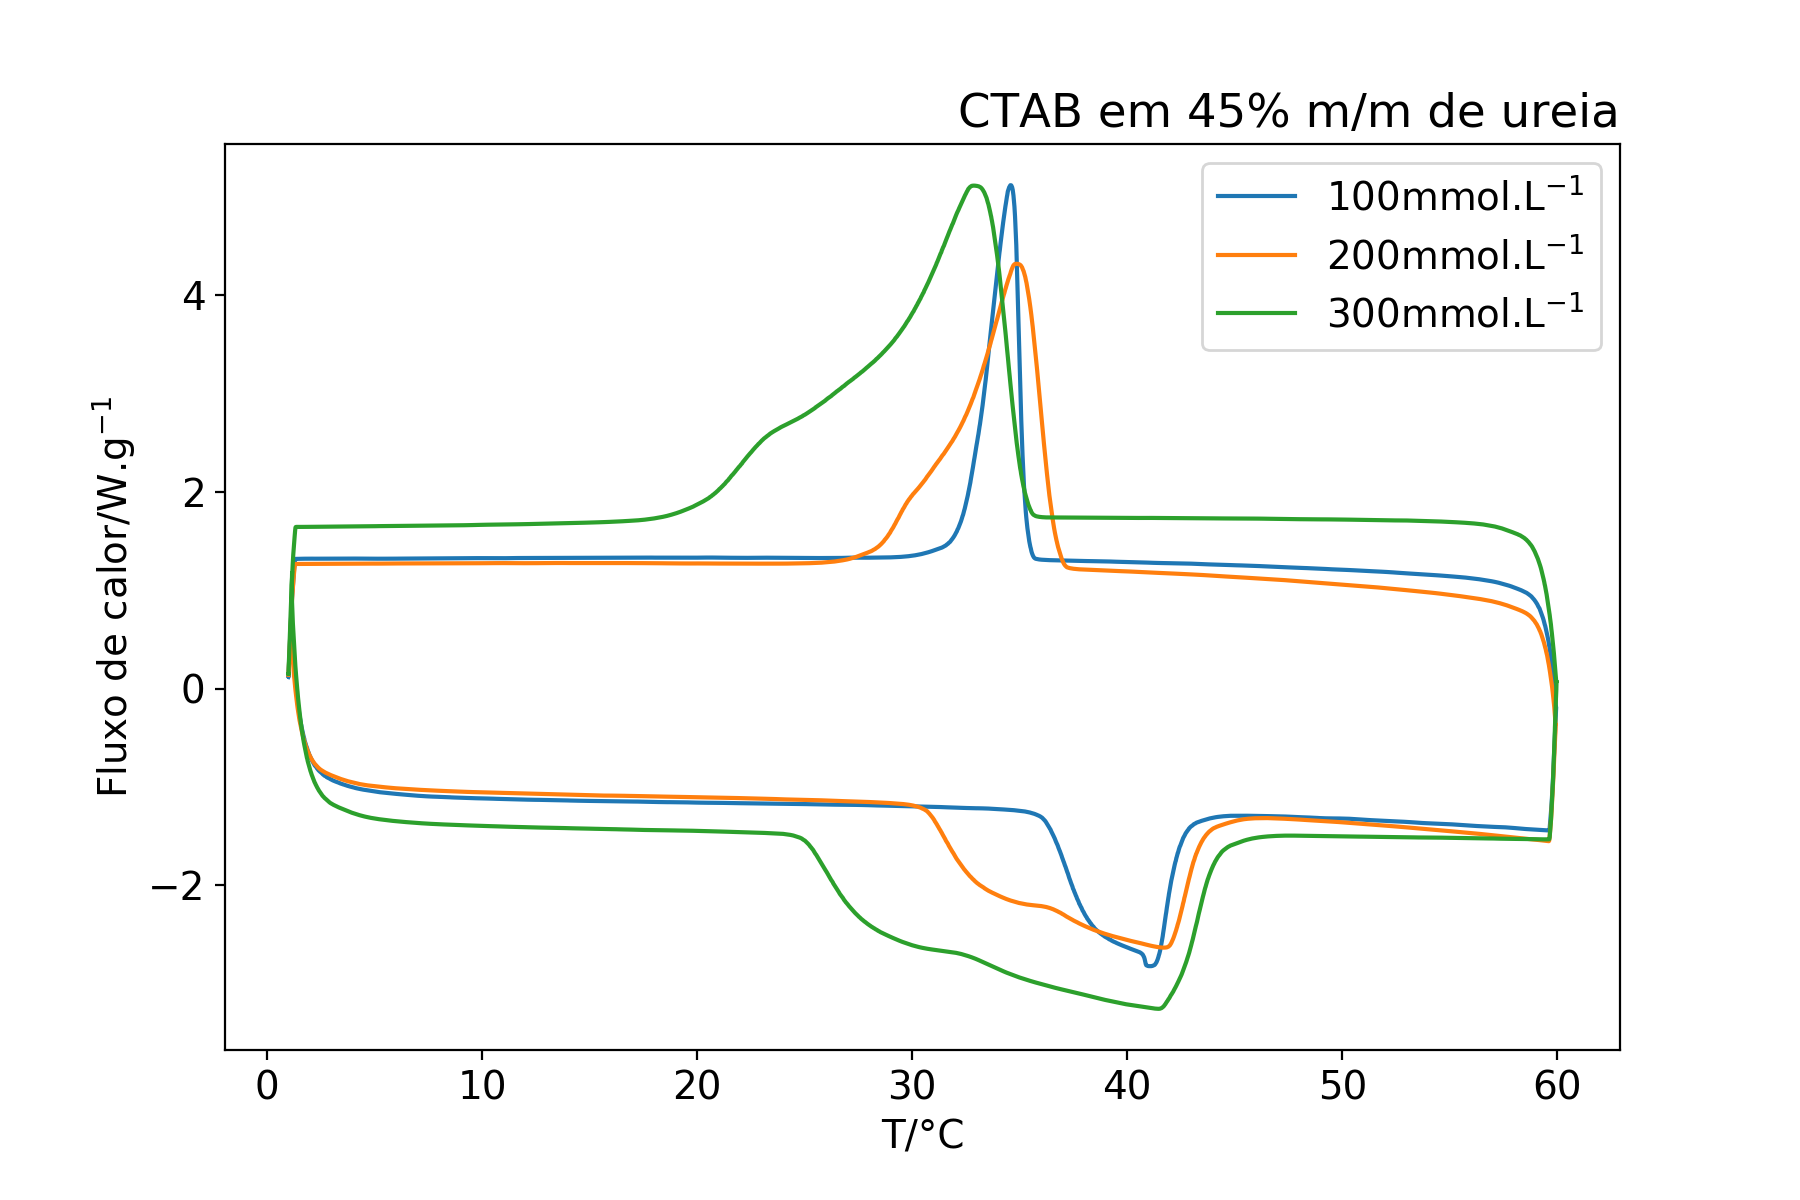
\includegraphics[width=\textwidth]{./imagens/dsc/CTAB_45p}
				\caption{45\% de ureia}
				\label{fig:DSC_CTAB_UR45}
			\end{subfigure} \qquad %
			\begin{subfigure}[h]{0.45\textwidth}
				\centering
				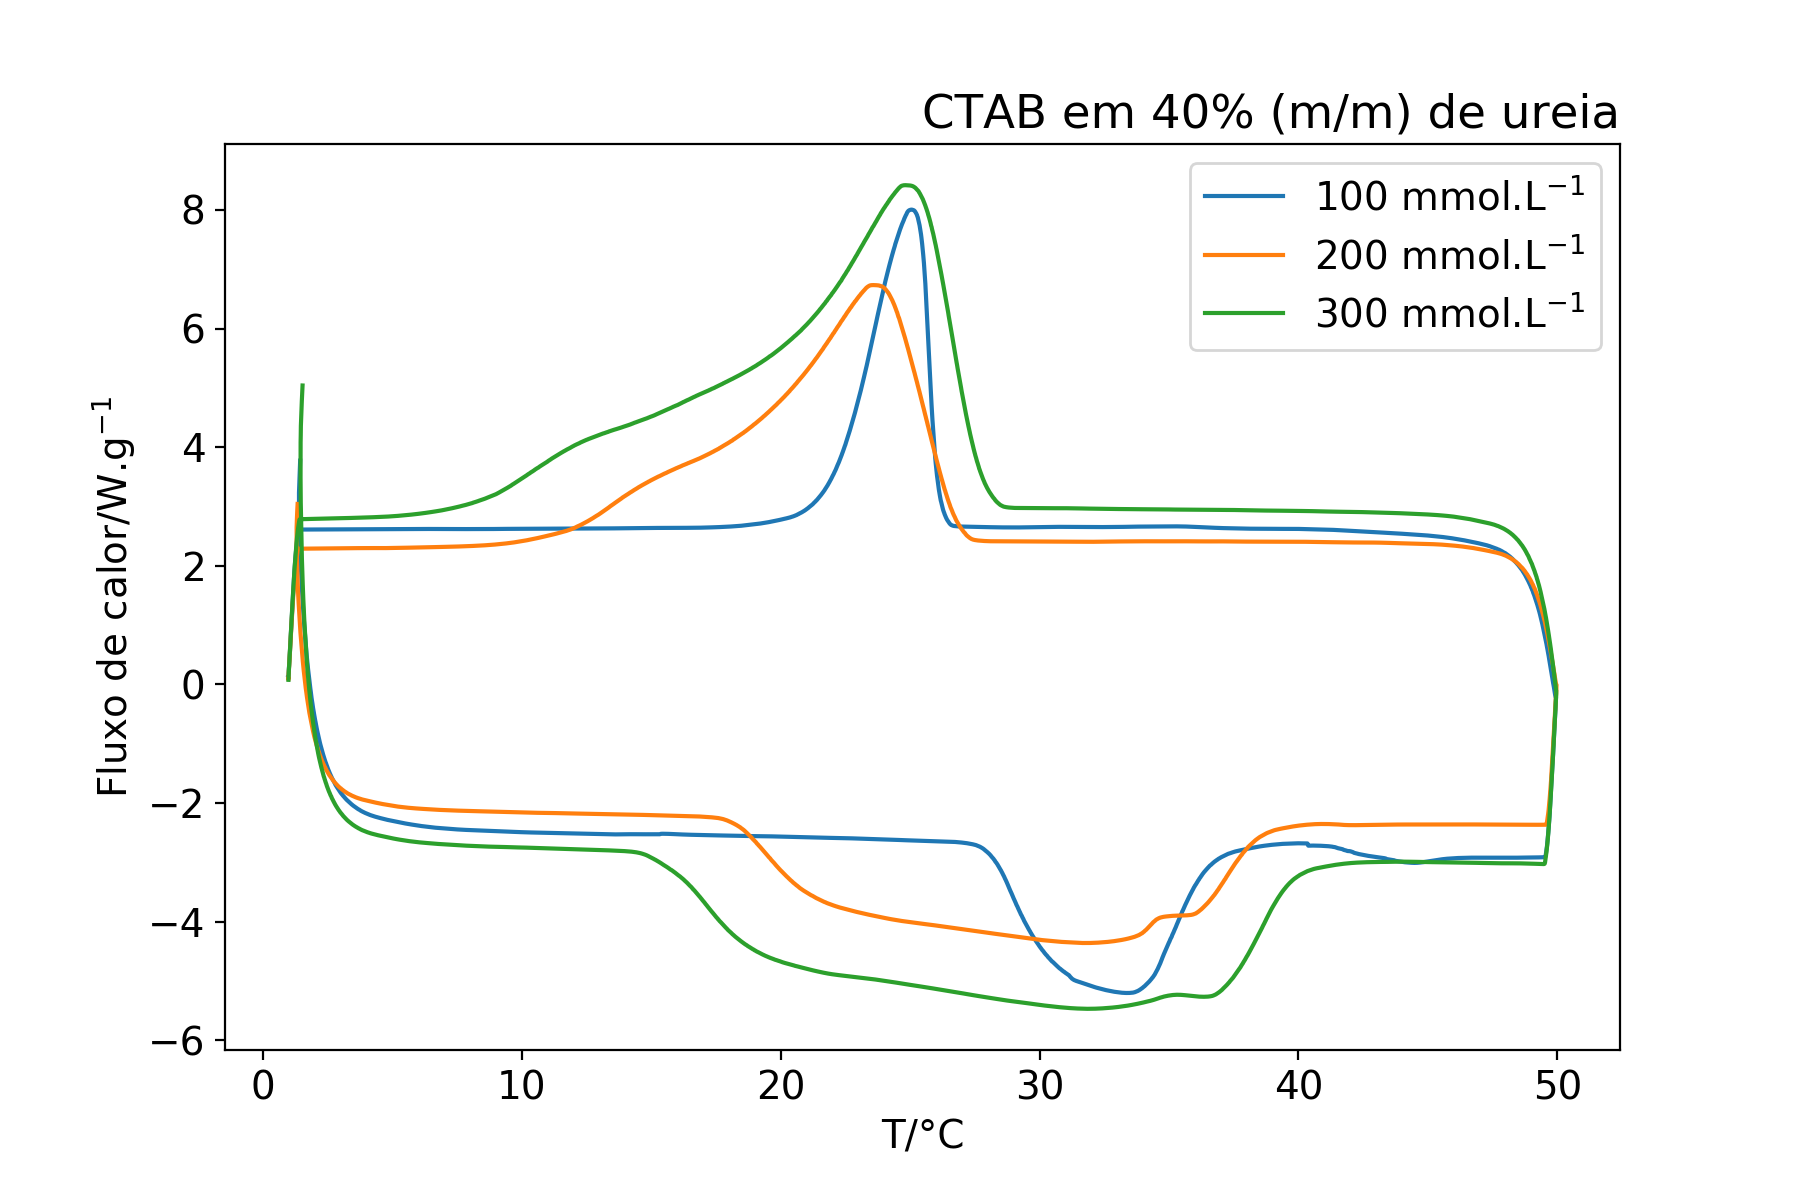
\includegraphics[width=\textwidth]{./imagens/dsc/CTAB_40p}
				\caption{40\% de ureia}
				\label{fig:DSC_CTAB_UR40}
			\end{subfigure}
			\caption{Termogramas de CTAB 100, 200 e 300 \mM{} em soluções em 45\% (\ref{fig:DSC_CTAB_UR45}) e 40\% (\ref{fig:DSC_CTAB_UR40})}
			\label{fig:DSC_CTAB_UR40-45}
		\end{figure}
	
		% todo: colocar o título da figura do 40% do lado direito
		\begin{figure}[h]
			\centering
			\begin{subfigure}[t]{0.45\textwidth}
				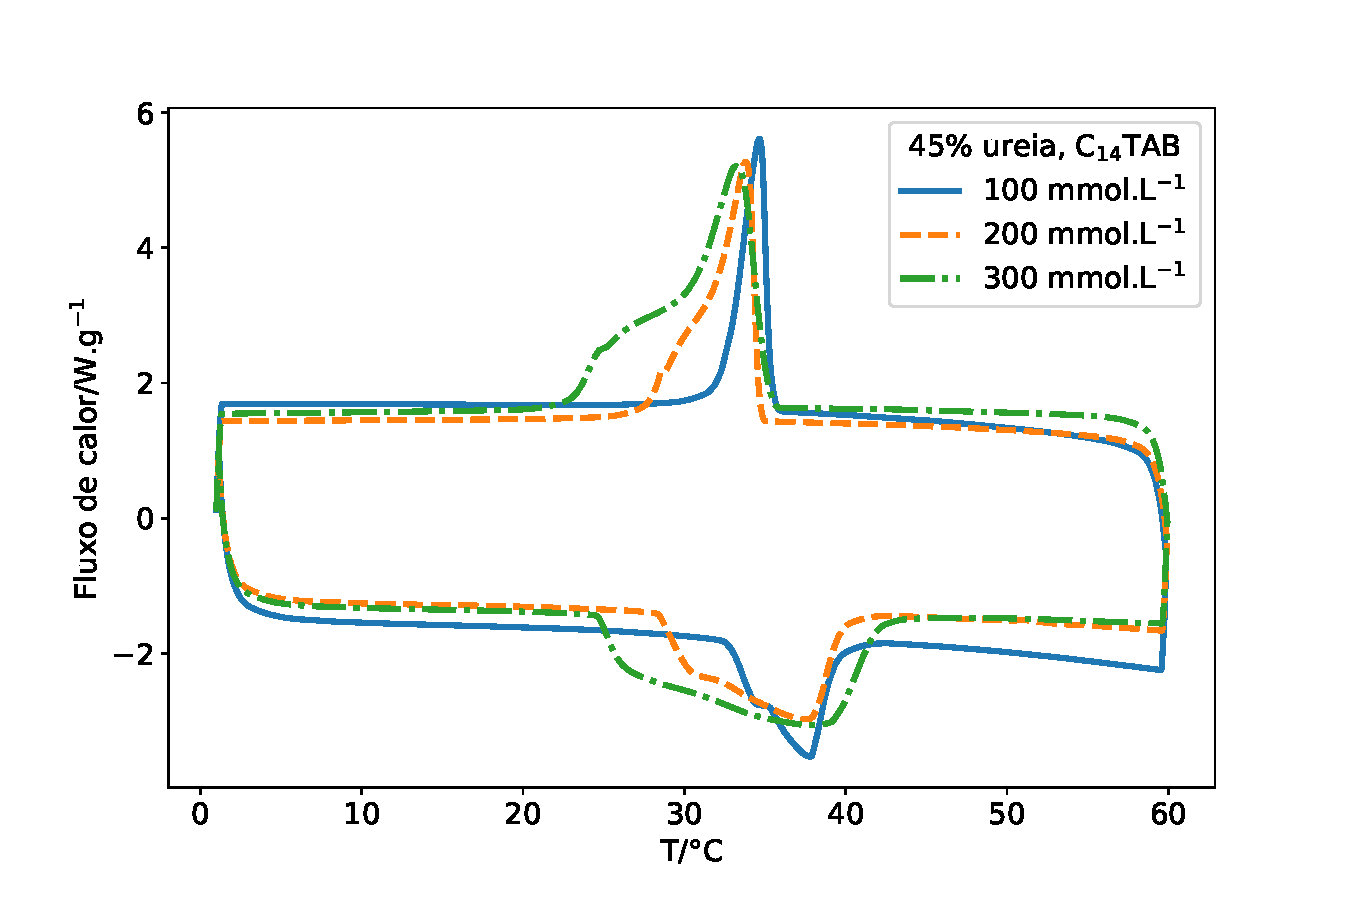
\includegraphics[width=\textwidth]{./imagens/dsc/TTAB_45p}
				\caption{45\% de ureia}
				\label{fig:DSC_TTAB_UR45}
			\end{subfigure} \qquad %
			\begin{subfigure}[t]{0.45\textwidth}
				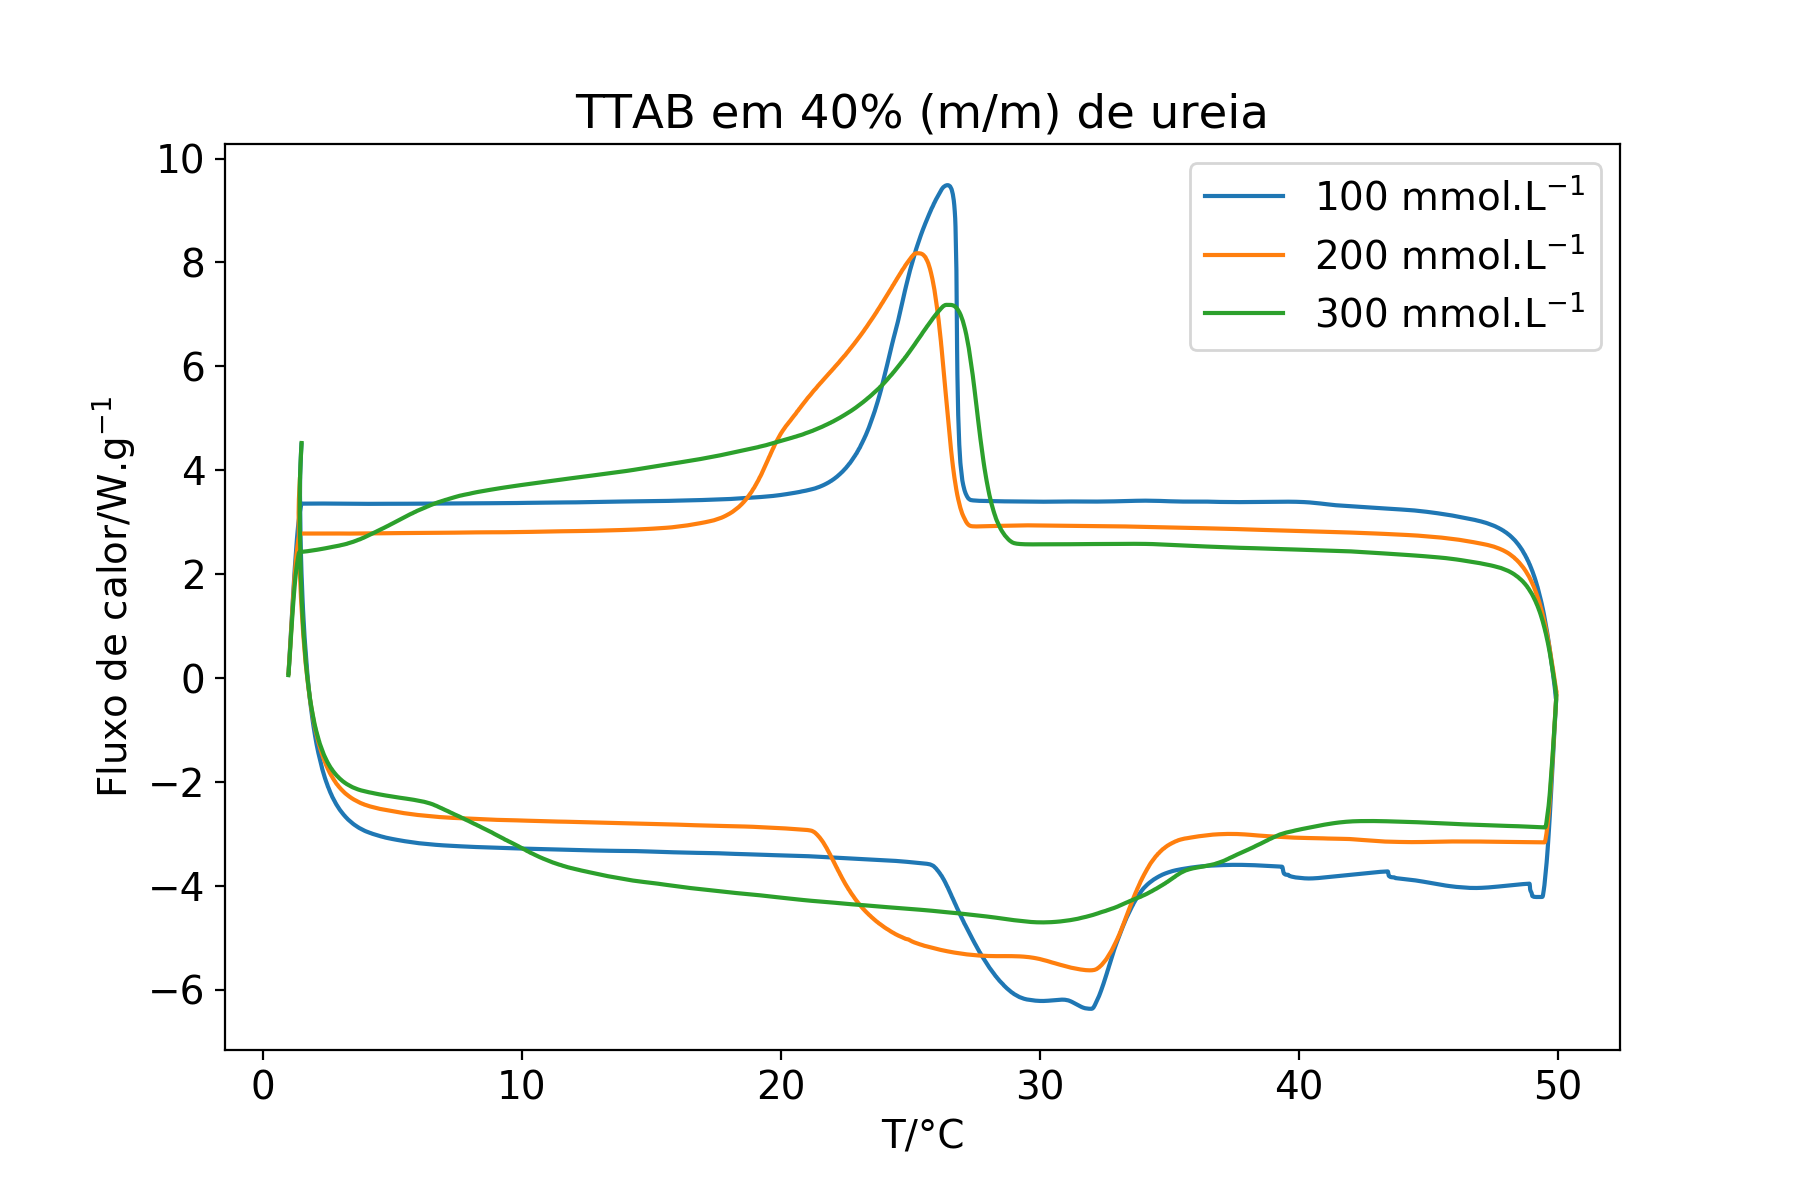
\includegraphics[width=\textwidth]{./imagens/dsc/TTAB_40p}
				\caption{40\% de ureia}
				\label{fig:DSC_TTAB_UR40}
			\end{subfigure}
			\caption{Termogramas de soluções de TTAB 100, 200 e 300 \mM{}, em 45\% (\ref{fig:DSC_TTAB_UR45}) e 40\% (\ref{fig:DSC_TTAB_UR40}) de ureia}
			\label{fig:DSC_TTAB_UR_40-45}
		\end{figure}
		
		\begin{figure}[h]
			\centering
			\begin{subfigure}[t]{0.45\textwidth}
				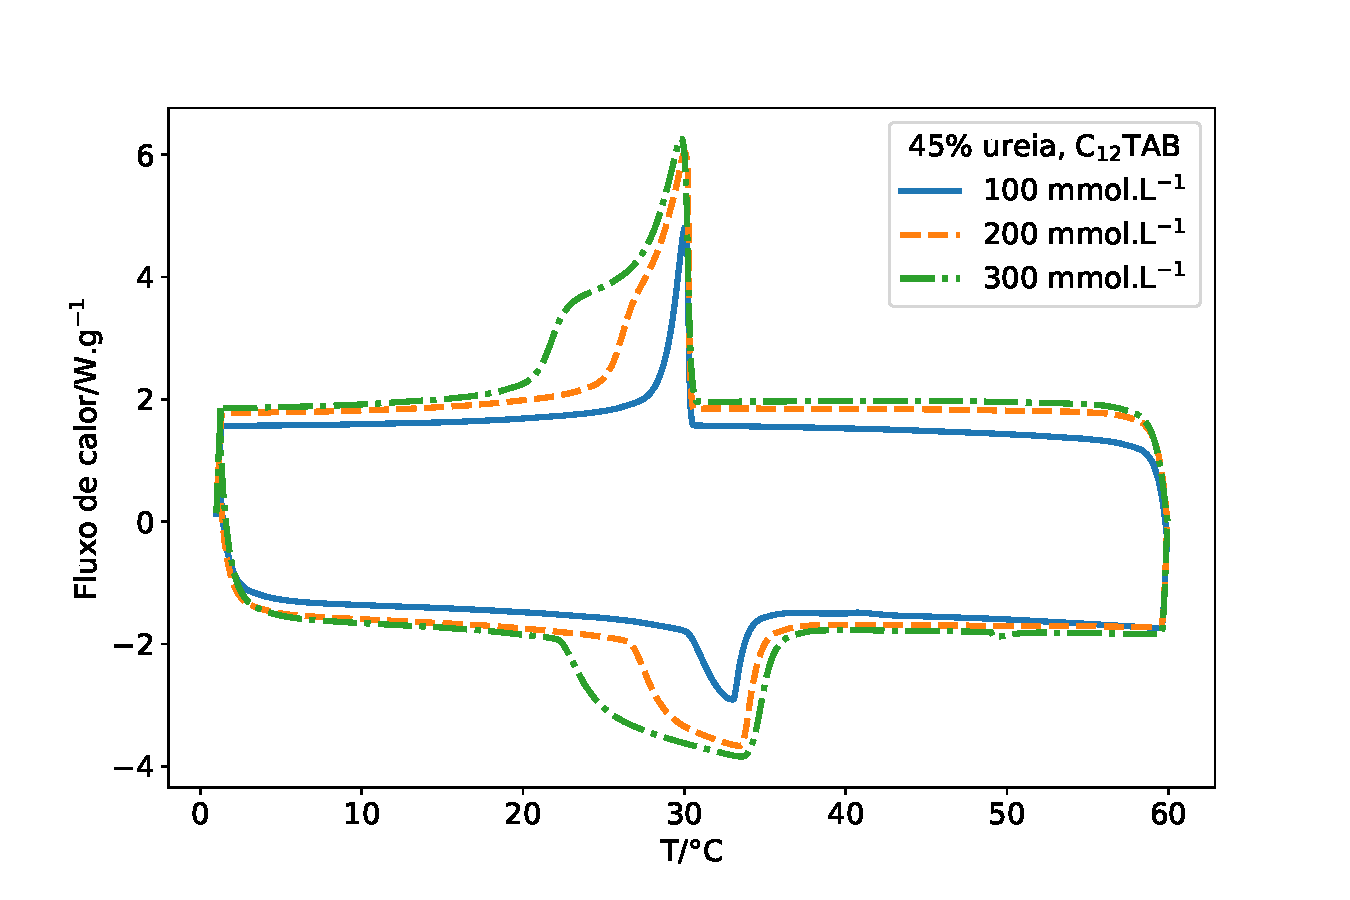
\includegraphics[width=\textwidth]{./imagens/dsc/DTAB_45p}
				\caption{45\% de ureia}
				\label{fig:DSC_DTAB_UR45}
			\end{subfigure} \qquad %
			\begin{subfigure}[t]{0.45\textwidth}
				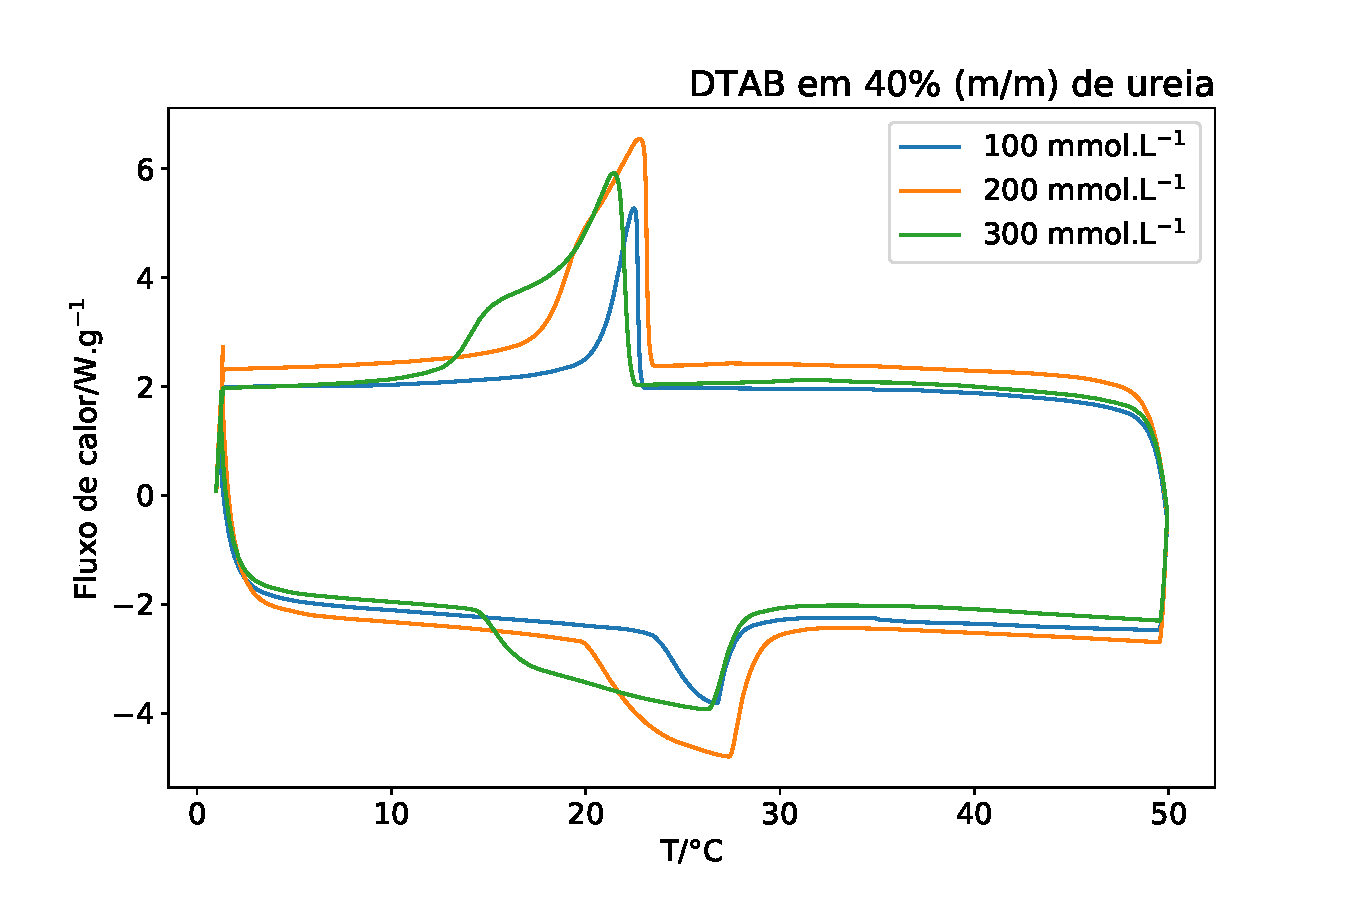
\includegraphics[width=\textwidth]{./imagens/dsc/DTAB_40p}
				\caption{40\% de ureia}
				\label{fig:DSC_DTAB_UR40}
			\end{subfigure}
			\caption{Termogramas de soluções de DTAB 100, 200 e 300 \mM{}, em 45\% (\ref{fig:DSC_DTAB_UR45}) e 40\% (\ref{fig:DSC_DTAB_UR40}) de ureia}
			\label{fig:DSC_DTAB_UR_40-45}
		\end{figure}
		
		
		% todo: verificar se a notação (C|T|D) é boa
		\begin{figure}[h]
			\centering
			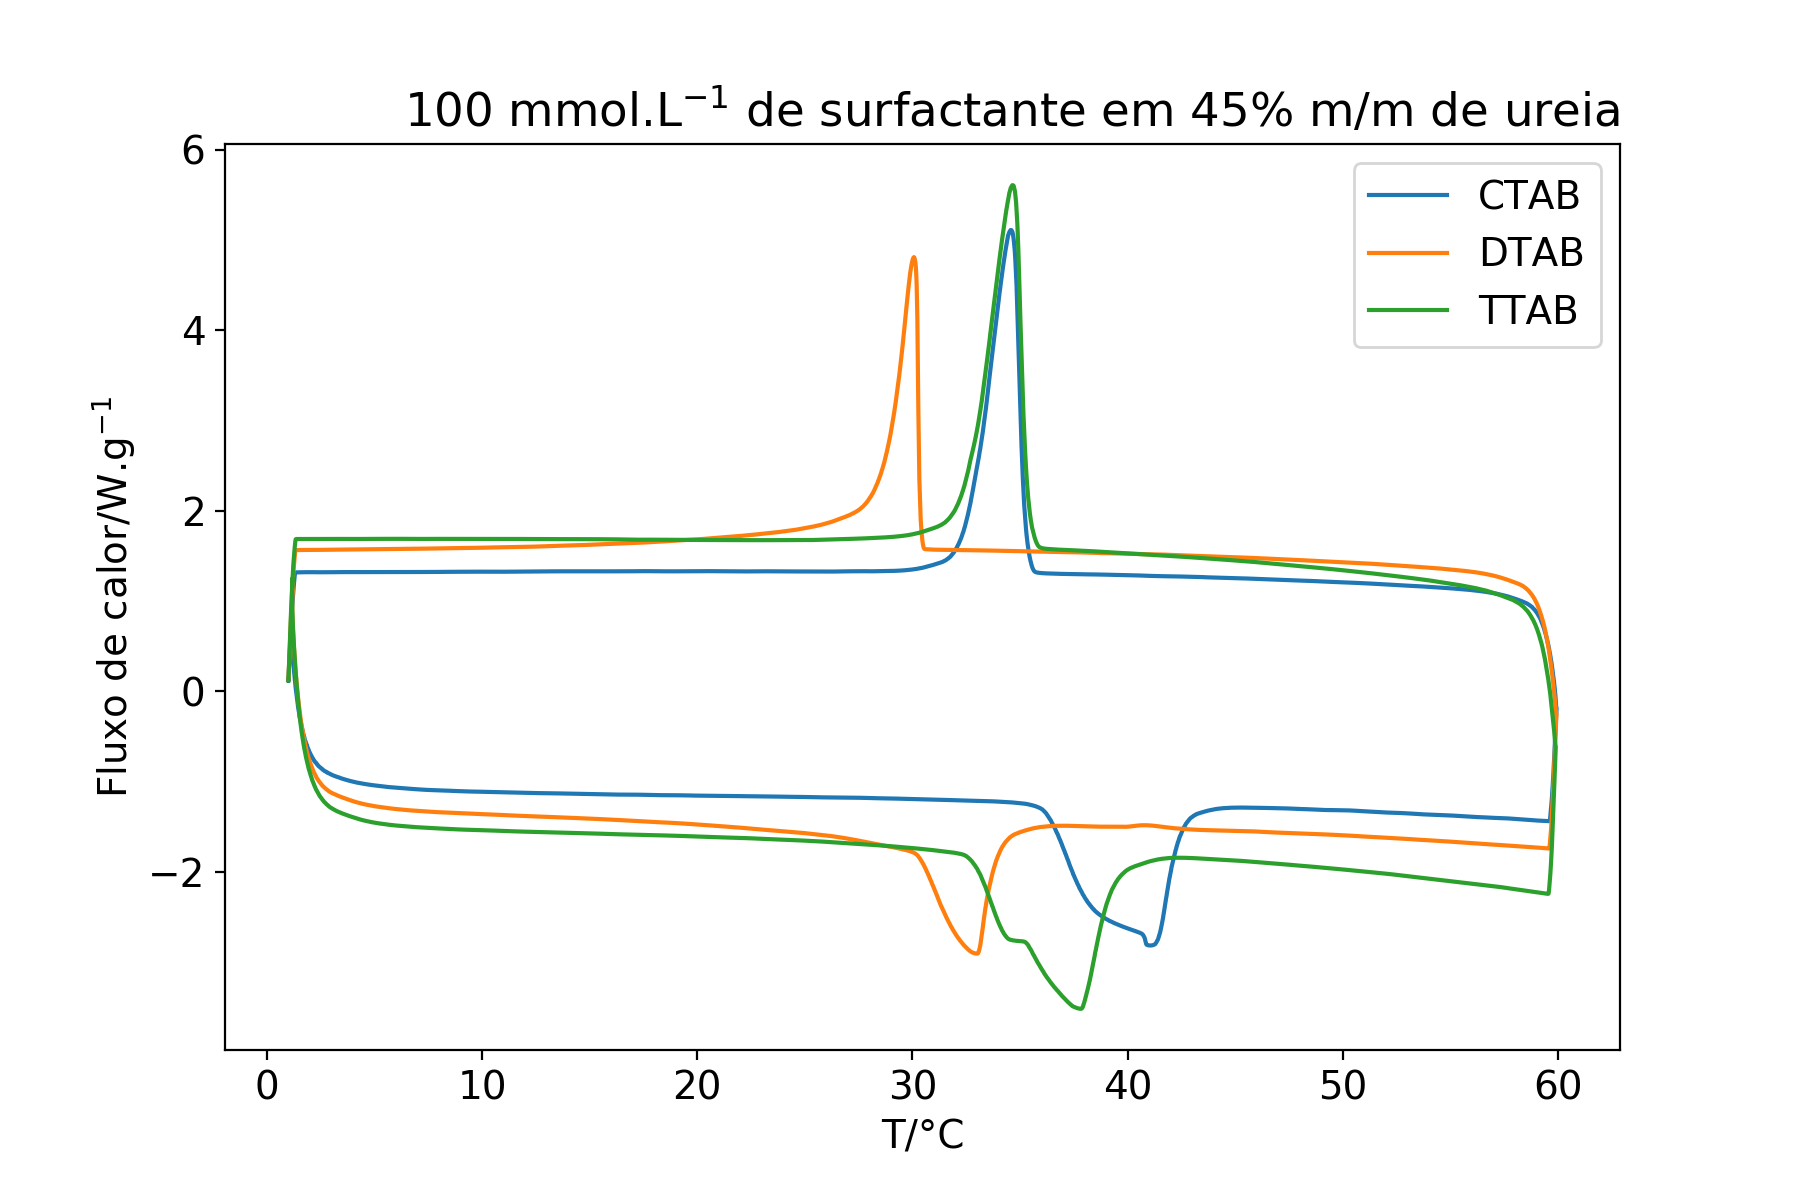
\includegraphics[width=0.45\textwidth]{./imagens/dsc/Surf_100mm_45p}
			\caption{Termogramas de soluções de (C|T|D)TAB 100 \mM{}, em 45\% de ureia}
			\label{fig:DSC_Surf_100mm_45p}
		\end{figure}
	
		\begin{figure}[h]
			\centering
			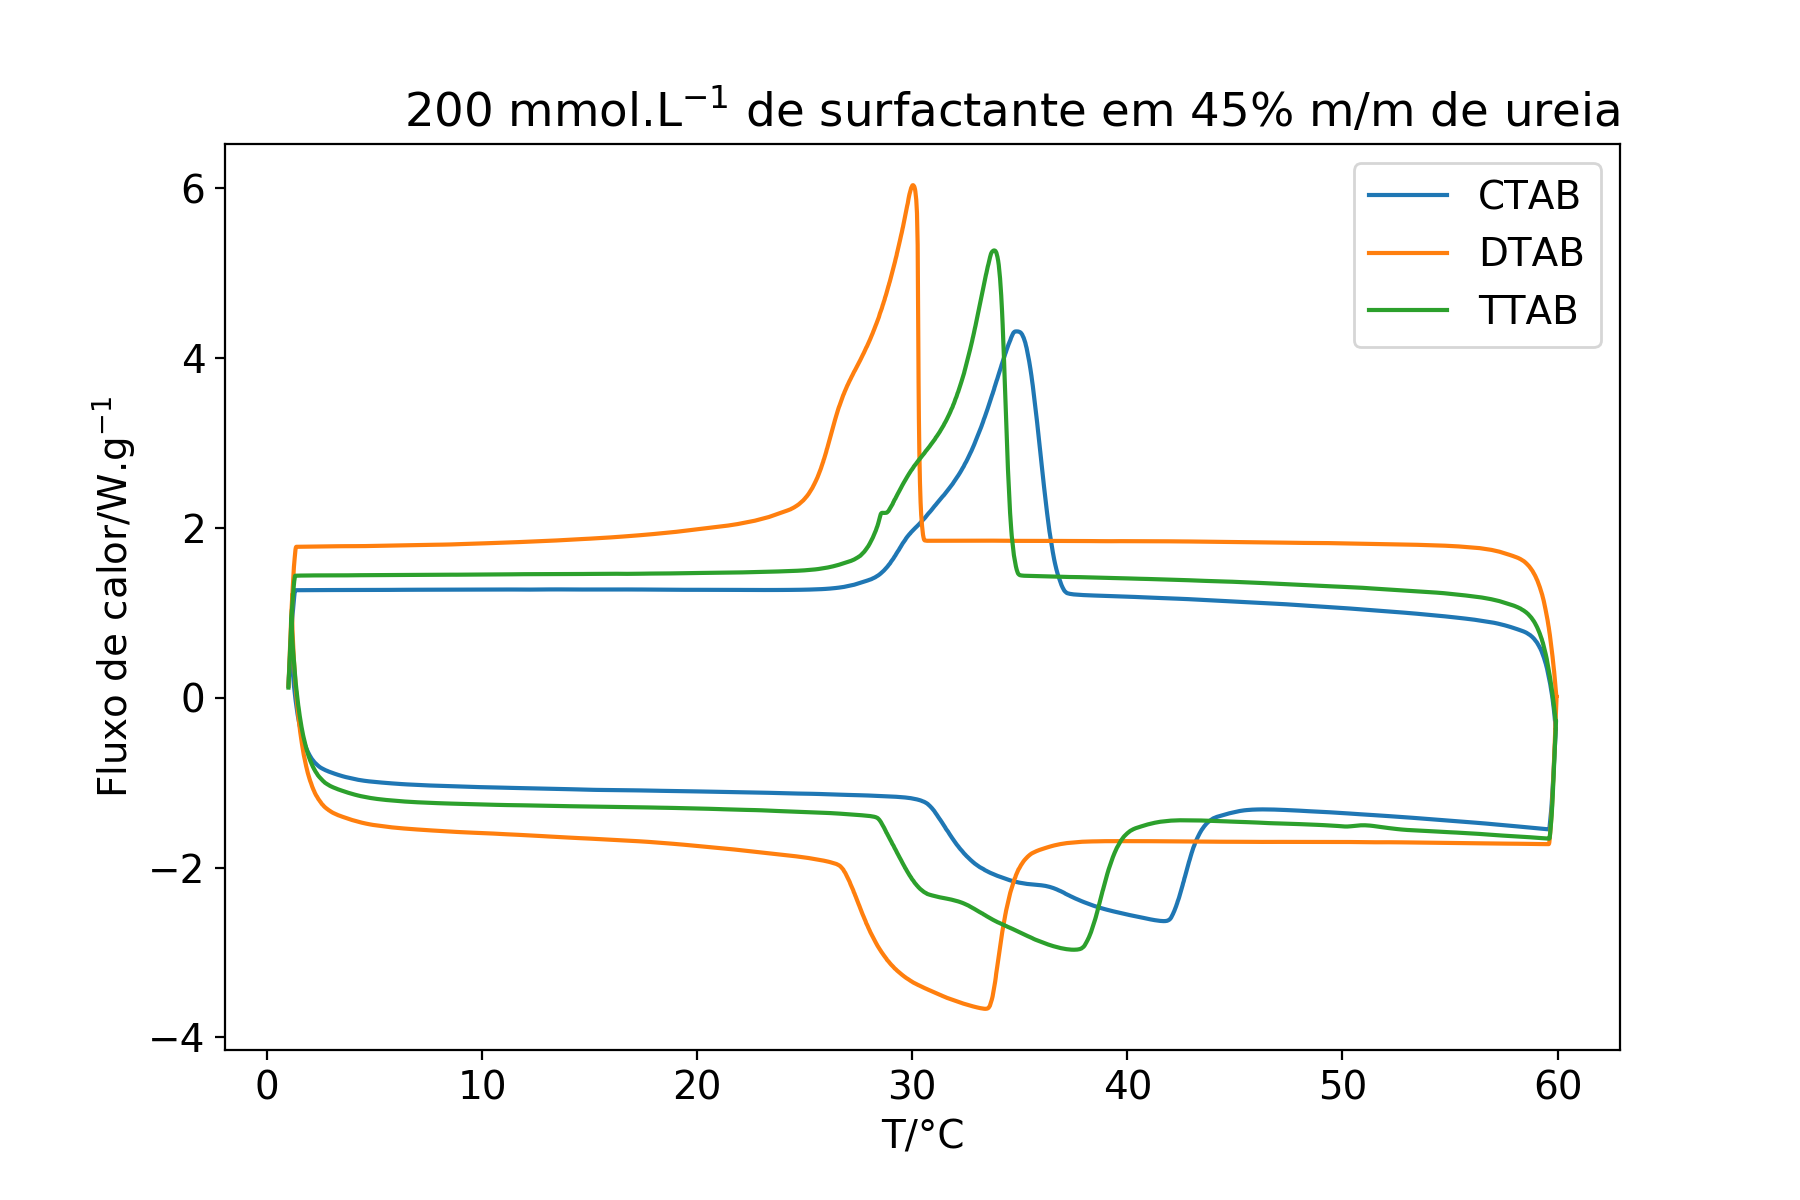
\includegraphics[width=0.45\textwidth]{./imagens/dsc/Surf_200mm_45p}
			\caption{Termogramas de soluções de (C|T|D)TAB 200 \mM{}, em 45\% de ureia}
			\label{fig:DSC_Surf_200mm_45p}
		\end{figure}
	
		\begin{figure}[h]
			\centering
			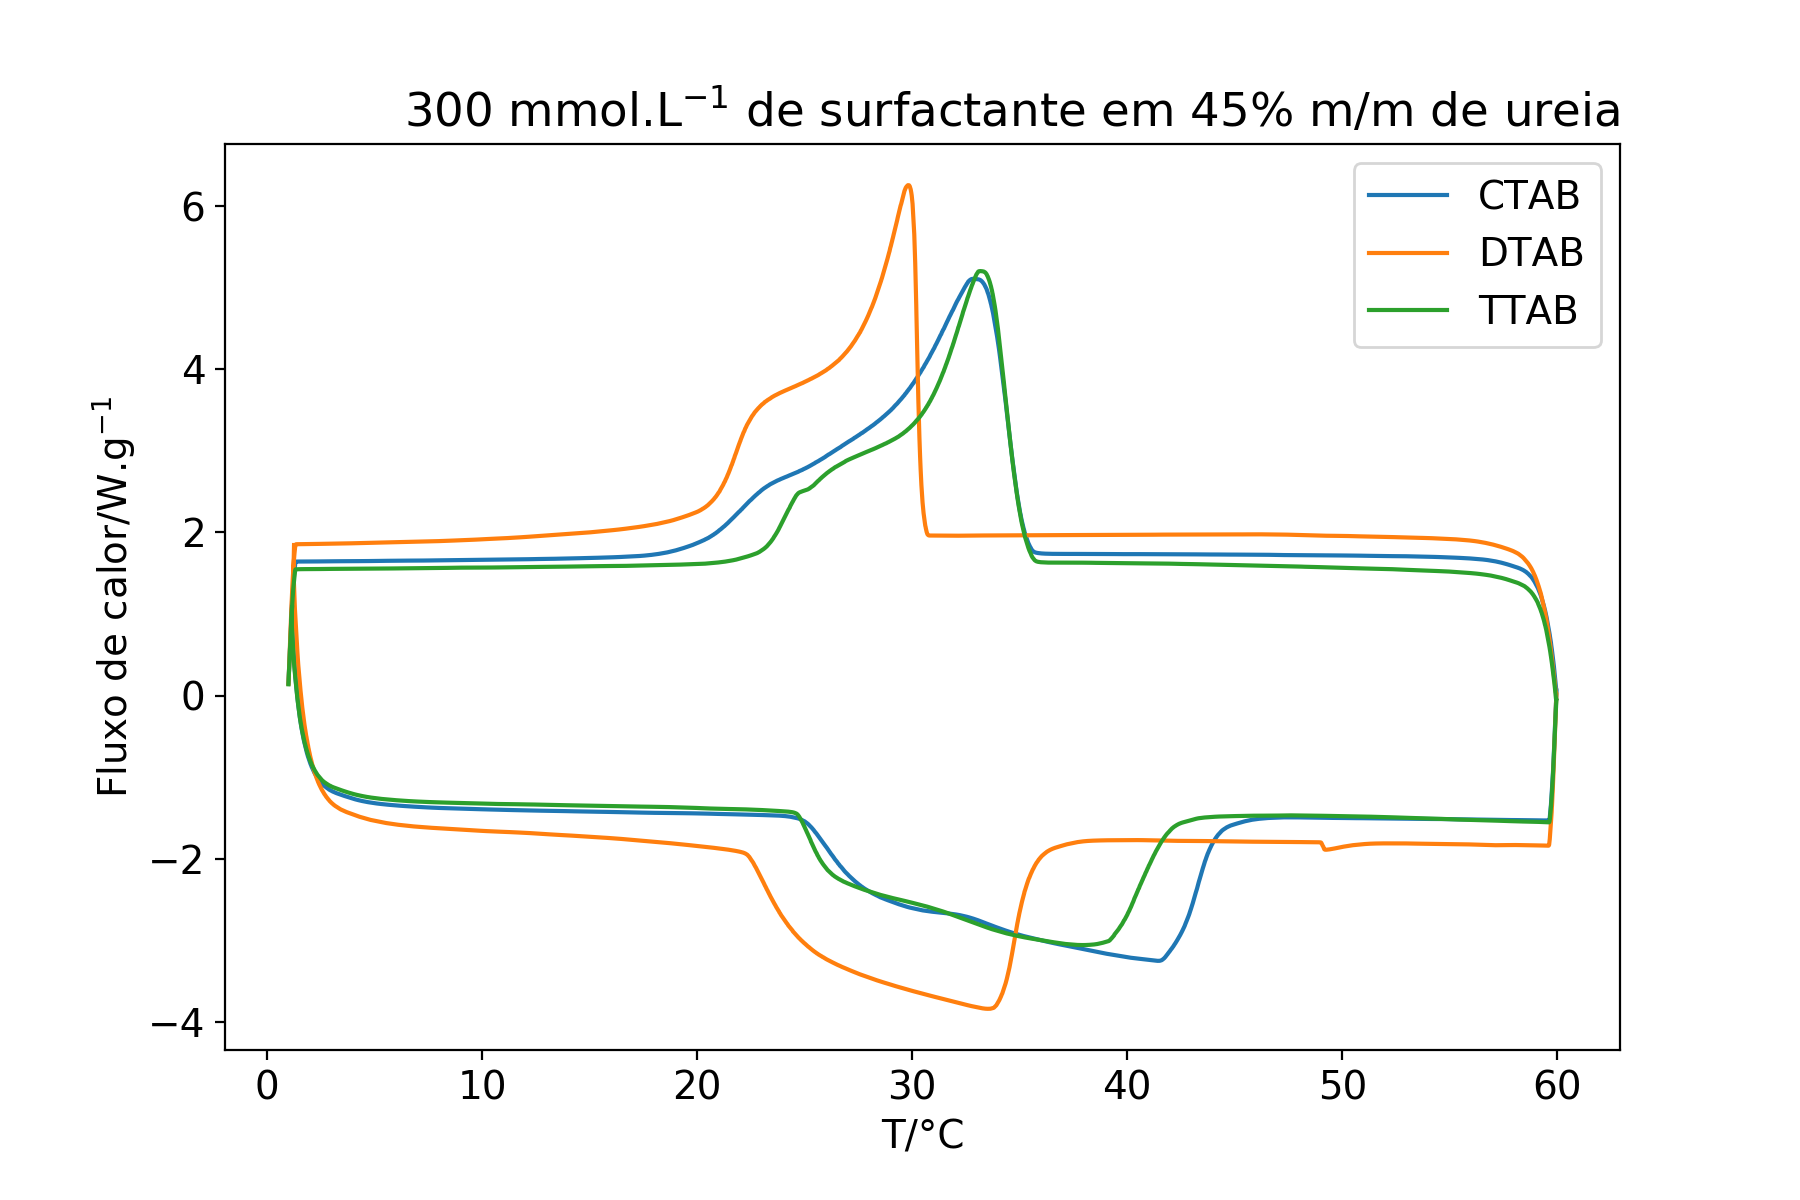
\includegraphics[width=0.45\textwidth]{./imagens/dsc/Surf_300mm_45p}
			\caption{Termogramas de soluções de (C|T|D)TAB 300 \mM{}, em 45\% de ureia}
			\label{fig:DSC_Surf_300mm_45p}
		\end{figure}
	
		%%%%%%%%% MG %%%%%%%%%%%%%%%%%%%%%
		% CTAB 100 NaSal 60: 35, 40, 45%
		% CTAB 100 NaSal 100: 35, 40, 45%
		% CTAB 100 NaSal 260: 35, 40, 45%
		%%%%%%%%%%%%%%%%%%%%%%%%%%%%%%%%%%
		
		% Efeito do tamanho da cadeia do surfactante	
		% CTAB, TTAB, DTAB; 100, 200, 300 a 45% ureia
		% CTAB, TTAB, DTAB; 100, 200, 300 a 40% ureia
		
		% Efeito da concentração de ureia
		% CTAB100 de 38% a 45% de ureia
		% CTAB300 de 38% a 45% de ureia (mandar fazer)
		% CTAB400 de 35%, 40%, 45%
		
	\section{SAXS}
	\section{DLS}
	\section{Reologia do sólido}
	\section{Entalpia de interação de ureia com surfactante}